
\documentclass[12pt]{article}\usepackage[]{graphicx}\usepackage[]{color}
%% maxwidth is the original width if it is less than linewidth
%% otherwise use linewidth (to make sure the graphics do not exceed the margin)
\makeatletter
\def\maxwidth{ %
  \ifdim\Gin@nat@width>\linewidth
    \linewidth
  \else
    \Gin@nat@width
  \fi
}
\makeatother

\definecolor{fgcolor}{rgb}{0.345, 0.345, 0.345}
\newcommand{\hlnum}[1]{\textcolor[rgb]{0.686,0.059,0.569}{#1}}%
\newcommand{\hlstr}[1]{\textcolor[rgb]{0.192,0.494,0.8}{#1}}%
\newcommand{\hlcom}[1]{\textcolor[rgb]{0.678,0.584,0.686}{\textit{#1}}}%
\newcommand{\hlopt}[1]{\textcolor[rgb]{0,0,0}{#1}}%
\newcommand{\hlstd}[1]{\textcolor[rgb]{0.345,0.345,0.345}{#1}}%
\newcommand{\hlkwa}[1]{\textcolor[rgb]{0.161,0.373,0.58}{\textbf{#1}}}%
\newcommand{\hlkwb}[1]{\textcolor[rgb]{0.69,0.353,0.396}{#1}}%
\newcommand{\hlkwc}[1]{\textcolor[rgb]{0.333,0.667,0.333}{#1}}%
\newcommand{\hlkwd}[1]{\textcolor[rgb]{0.737,0.353,0.396}{\textbf{#1}}}%
\let\hlipl\hlkwb

\usepackage{framed}
\makeatletter
\newenvironment{kframe}{%
 \def\at@end@of@kframe{}%
 \ifinner\ifhmode%
  \def\at@end@of@kframe{\end{minipage}}%
  \begin{minipage}{\columnwidth}%
 \fi\fi%
 \def\FrameCommand##1{\hskip\@totalleftmargin \hskip-\fboxsep
 \colorbox{shadecolor}{##1}\hskip-\fboxsep
     % There is no \\@totalrightmargin, so:
     \hskip-\linewidth \hskip-\@totalleftmargin \hskip\columnwidth}%
 \MakeFramed {\advance\hsize-\width
   \@totalleftmargin\z@ \linewidth\hsize
   \@setminipage}}%
 {\par\unskip\endMakeFramed%
 \at@end@of@kframe}
\makeatother

\definecolor{shadecolor}{rgb}{.97, .97, .97}
\definecolor{messagecolor}{rgb}{0, 0, 0}
\definecolor{warningcolor}{rgb}{1, 0, 1}
\definecolor{errorcolor}{rgb}{1, 0, 0}
\newenvironment{knitrout}{}{} % an empty environment to be redefined in TeX

\usepackage{alltt}
\usepackage{mathpazo}
\usepackage[breaklinks=true]{hyperref}
\usepackage{url}
\usepackage[a4paper,margin=1.5cm]{geometry}
\usepackage{a4wide}
\usepackage{float}
\usepackage[english]{babel}
\usepackage[utf8]{inputenc}
\usepackage{amsmath}
\usepackage{amssymb}
\usepackage{color}
\usepackage[backend=bibtex,style=numeric-comp,sorting=none]{biblatex}
\bibliography{papers}
\usepackage{subcaption}
\usepackage[font={small}]{caption}
\usepackage{booktabs}
\usepackage{listings}
\usepackage{tikz}
\usetikzlibrary{decorations, matrix, arrows, shapes, positioning, calc, fit}
\tikzset
{
  mybox/.style={draw, minimum height=.8cm, minimum width=.9cm},
  myflip/.style={draw, fill=gray!30, minimum height=.8cm, minimum width=.9cm},
  myint/.style={draw, minimum height=.8cm, minimum width=1.1cm},
  mynone/.style={draw=none}
}

\usepackage{graphicx,epstopdf}
\epstopdfsetup{update} % only regenerate pdf files when eps file is newer
\usepackage{cleveref}
\usepackage{collcell} % loads array
\newcolumntype{m}{>{$} r <{$}}
\newcolumntype{u}{>{$[\collectcell\si} l <{\endcollectcell]$}}
\newcommand{\approxtext}[1]{\ensuremath{\stackrel{\text{#1}}{=}}}
\newcommand{\matr}[1]{\mathbf{#1}}
\newcommand{\partt}[2]{\ensuremath{\dfrac{\partial {#1}}{\partial {#2}}}}
\renewcommand{\d}[1]{\ensuremath{\operatorname{d}\!{#1}}} % non-italized differentials
\newcommand{\h}[0]{\ensuremath{\hbar}} % hbar
\newcommand{\qed}[0]{\ensuremath{\tag*{$\square$}}} % QED square
\def\changemargin#1#2{\list{}{\rightmargin#2\leftmargin#1}\item[]}
\let\endchangemargin=\endlist 
\usepackage{amsthm}
\theoremstyle{plain}
\newtheorem{thm}{theorem} % reset theorem numbering for each chapter
\theoremstyle{definition}
\newtheorem{defn}[thm]{definition} % definition numbers are dependent on theorem numbers
\newtheorem{exmp}[thm]{example} % same for example numbers
\renewcommand{\theequation}{\thesection.\arabic{equation}}
\def\changemargin#1#2{\list{}{\rightmargin#2\leftmargin#1}\item[]}
\let\endchangemargin=\endlist    
\newcommand{\ts}{\textsuperscript} 
\title
{
  \phantom{a}\vspace{2cm}
	\textbf
	{
      Scientific Programming: Assignment 1
  }\\[1em]
  \small{University of Cambridge}
}

\author{Henrik Åhl}
\date{\today}

% Stephen's stuff
\newcommand{\R}{\texttt{R}}
\newcommand{\Rfunction}[1]{{\texttt{#1}}}
\newcommand{\Robject}[1]{{\texttt{#1}}}
\newcommand{\Rpackage}[1]{{\mbox{\normalfont\textsf{#1}}}}
\usepackage{xcolor}
\definecolor{Red}{rgb}{0.7,0,0}
\definecolor{Blue}{rgb}{0,0,0.8}
\definecolor{Green}{rgb}{0,.8,0}
\hypersetup{%
  pdfusetitle,
  bookmarks = {true},
  bookmarksnumbered = {true},
  bookmarksopen = {true},
  bookmarksopenlevel = 2,
  unicode = {true},
  breaklinks = {false},
  hyperindex = {true},
  colorlinks = {true},
  linktocpage = {true},
  plainpages = {false},
  linkcolor = {Blue},
  citecolor = {Blue},
  urlcolor = {Red},
  pdfstartview = {Fit},
  pdfpagemode = {UseOutlines},
  pdfview = {XYZ null null null}
}
%% Listings
\lstset{ 
  language=R,                     % the language of the code
  basicstyle=\footnotesize,       % the size of the fonts that are used for the code
  numbers=left,                   % where to put the line-numbers
  numberstyle=\tiny\color{gray},  % the style that is used for the line-numbers
  stepnumber=1,                   % the step between two line-numbers. If it's 1, each line will be numbered
  numbersep=5pt,                  % how far the line-numbers are from the code
  backgroundcolor=\color{white},  % choose the background color. You must add \usepackage{color}
  showspaces=false,               % show spaces adding particular underscores
  showstringspaces=false,         % underline spaces within strings
  showtabs=false,                 % show tabs within strings adding particular underscores
  rulecolor=\color{black},        % if not set, the frame-color may be changed on line-breaks within not-black text (e.g. commens (green here))
  tabsize=2,                      % sets default tabsize to 2 spaces
  captionpos=b,                   % sets the caption-position to bottom
  breaklines=true,                % sets automatic line breaking
  breakatwhitespace=false,        % sets if automatic breaks should only happen at whitespace
  title=\lstname,                 % show the filename of files included with \lstinputlisting;
                                  % also try caption instead of title
  keywordstyle=\color{Blue},      % keyword style
  commentstyle=\color{Green},     % comment style
  stringstyle=\color{Red},        % string literal style
  escapeinside={\%*}{*)},         % if you want to add a comment within your code
  morekeywords={*,...}            % if you want to add more keywords to the set
} 
\usepackage{verbatim}
\IfFileExists{upquote.sty}{\usepackage{upquote}}{}
\begin{document}
\date{\today}
\maketitle

\newpage
\section{Introduction}

This is an assignment report in connection to the \textit{Scientific Programming with \R} module in the Computational Biology course at the University of Cambridge, Michelmas term 2016. All related code is as of \date{\today} available on \url{https://github.com/supersubscript/compbio/tree/master/src/sp_assignments/assignment_1}, or available per request by contacting \href{mailto:hpa22@cam.ac.uk}{hpa22@cam.ac.uk}. Likewise, the corresponding assignment can be found on \url{https://github.com/sje30/rpc2016/tree/master/assigns}.


\section{Solutions}
The assignment consists of three sections, related to various parts of scientific programming. The first section deals with geometric plotting, the second with developing an algorithm for solving cryptarithms, and the third with data manipulation and visualisation. 

\subsection{Curved Squares}
\begin{figure}[H]
  \centering
  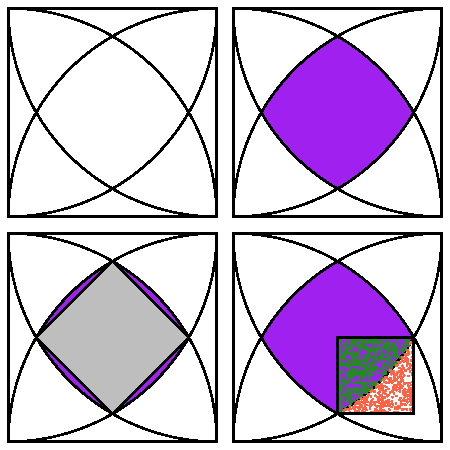
\includegraphics[scale=.7]{curved_squares.pdf}
  \caption{The arcs and corresponding geometries, as well as the area estimate.}
\end{figure}

The analytic area can be derived by tracing the two upper quarter circles to their intersection and realising that a triangle based in the two bottom corners and this point must be equilateral. We can then use two sides of the triangle to form a circle sector, which must have area $\pi/6$. Likewise, we can use the triangle to extract a circle segment, which correspondingly will have area $\pi/6 - \sin(\pi/3)/2$. Knowing that a full quarter circle is here of area $pi/4$, we can easily deduce that the area surrounding the shape must be four times the area of the circle quartile minus the segment and sector. \textit{Summa sumarum}, we find that the enclosed area is
\begin{align*}
  1 - (\pi/4 - \pi/6 - (\pi/6 - \sin(\pi/3)/2)) \approx 0.315\text{.}
\end{align*}
\begin{center}
  \lstinputlisting[float=h,language={}, tabsize = 4]{curved_squares_out.txt}
\end{center}
\subsection{Cryptarithms}
This exercise was solved using matrix manipulations, inserting character columns from a letter-value permutation matrix, parsing and evaluating. It has an approximate runtime on the order of minutes.
\lstinputlisting[float=h,language={}, tabsize = 4]{cryptarithms_out.txt}

\subsection{Word Processing}
In the word processing part, $y$ is treated as a vowel (as it should be). The dictionary does not distinguish between capitalised letters or not, so in particular in the palindrome exercise, the palindromes will be replicated if variants with different capitalisations exist. 
\begin{center}
  \lstinputlisting[language={}]{word_processing_out.txt}
  \lstinputlisting[language={}]{word_processing_noVowelWords.txt}
  \lstinputlisting[language={}]{word_processing_palindromes.txt}
\end{center}

\begin{figure}[H]
  \centering
  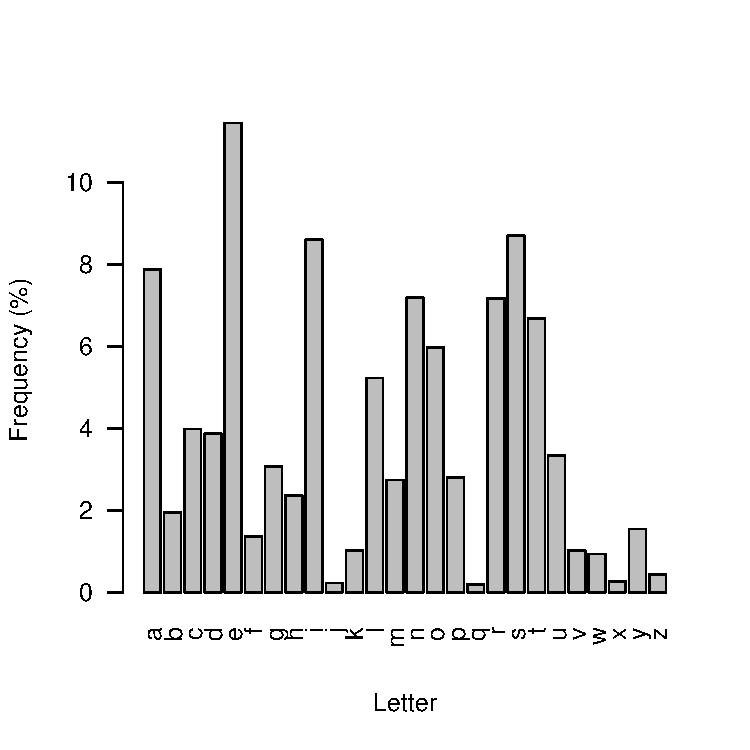
\includegraphics[scale=.7]{word_processing_letter_frequency.pdf}
  \caption{Letter frequencies for the Ubuntu English (UK) dictionary.}
\end{figure}
\begin{figure}[H]
  \centering
  \hspace{-2cm}
  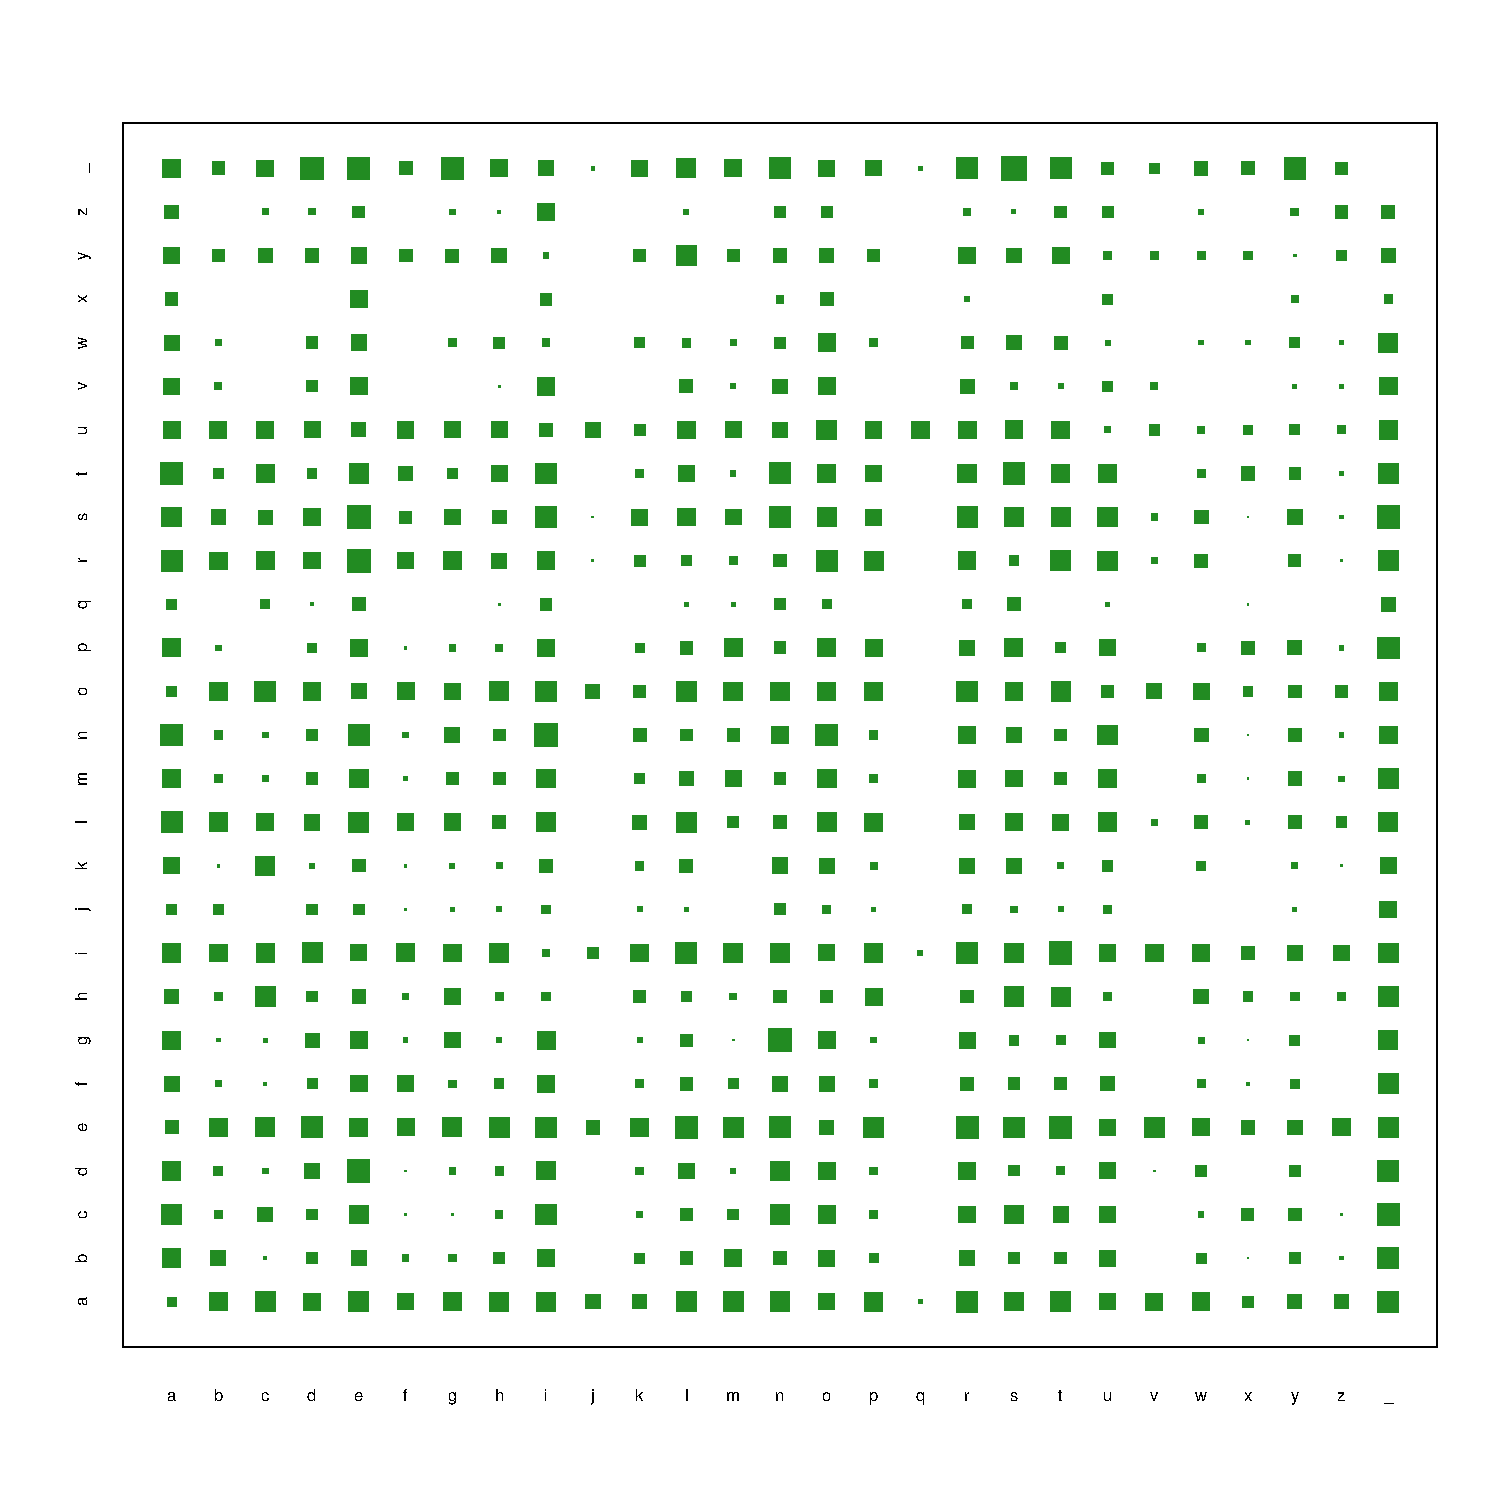
\includegraphics[scale=.7]{word_processing_bigram.pdf}
  \caption{Bigram for the letters contained in the dictionary. Square areas are proportional to the logarithm of the number of occurences.     The horizontal row marks the first character, the vertical the subsequent. (You said frequency in the exercise, but I think log(occ) makes   more sense for visualisation.)}
\end{figure}

\newpage
\section*{Code}
  \begin{center}
    \lstinputlisting{../../../src/sp_assignments/assignment_1/curved_squares.R}
    \lstinputlisting{../../../src/sp_assignments/assignment_1/cryptarithms.R}
    \lstinputlisting{../../../src/sp_assignments/assignment_1/word_processing.R}
  \end{center}
\end{document}

